%Stephen Stengel
%Cookies

\documentclass[12pt, letterpaper]{article}
\usepackage[utf8]{inputenc}
\usepackage{siunitx}
\usepackage{graphicx}
\usepackage{float} %placing figures with H

\begin{document}
\thispagestyle{empty}
\twocolumn

\begin{flushleft}
\section*{Stephen's Cookies}
\subsection*{Ingredients}
Metric weights are within $\pm$ 0.5g.

\begin{itemize}
\item 150g flour
\item 10g baking soda
\item 2g salt
\item a dash of curry powder or turmeric
\item 1 stick of soy butter (about 111g), cold
\item 70g brown sugar
\item 1 whole egg, (about 45 to 50g)
\item 1 egg yolk, (about 15 to 20g)
\item 3g vanilla extract
\item 154g dark chocolate, chips or broken bar pieces.
\end{itemize}

\subsection*{Instructions}
\begin{enumerate}
\item Preheat oven to \SI{375}{\degree}F. You will need two salad bowls.
\item Mix flour, baking soda, salt, and turmeric in one bowl.
\item Mix sugar, molasses, butter, eggs, and vanilla in a second bowl.
\item Mix the first bowl into the second bowl.
\item Mix in the chocolate chips.
\item Arrange on cookie sheet.
\item Bake for 15 minutes.
\end{enumerate}


\subsection*{Notes}
Makes about 13 cookies. These should be soft, bready, and not as sweet as most cookies. Do not butter or grease the baking pan. This recipe is the current best batch that I have made. To make more crumbly, buttery cookies, reduce flour to 100g.

%~ HEY: Test with non-brown sugar, brown sugar is just sugar with molasses in it.

%~ Update picture.

\begin{figure}[H]
\begin{center}
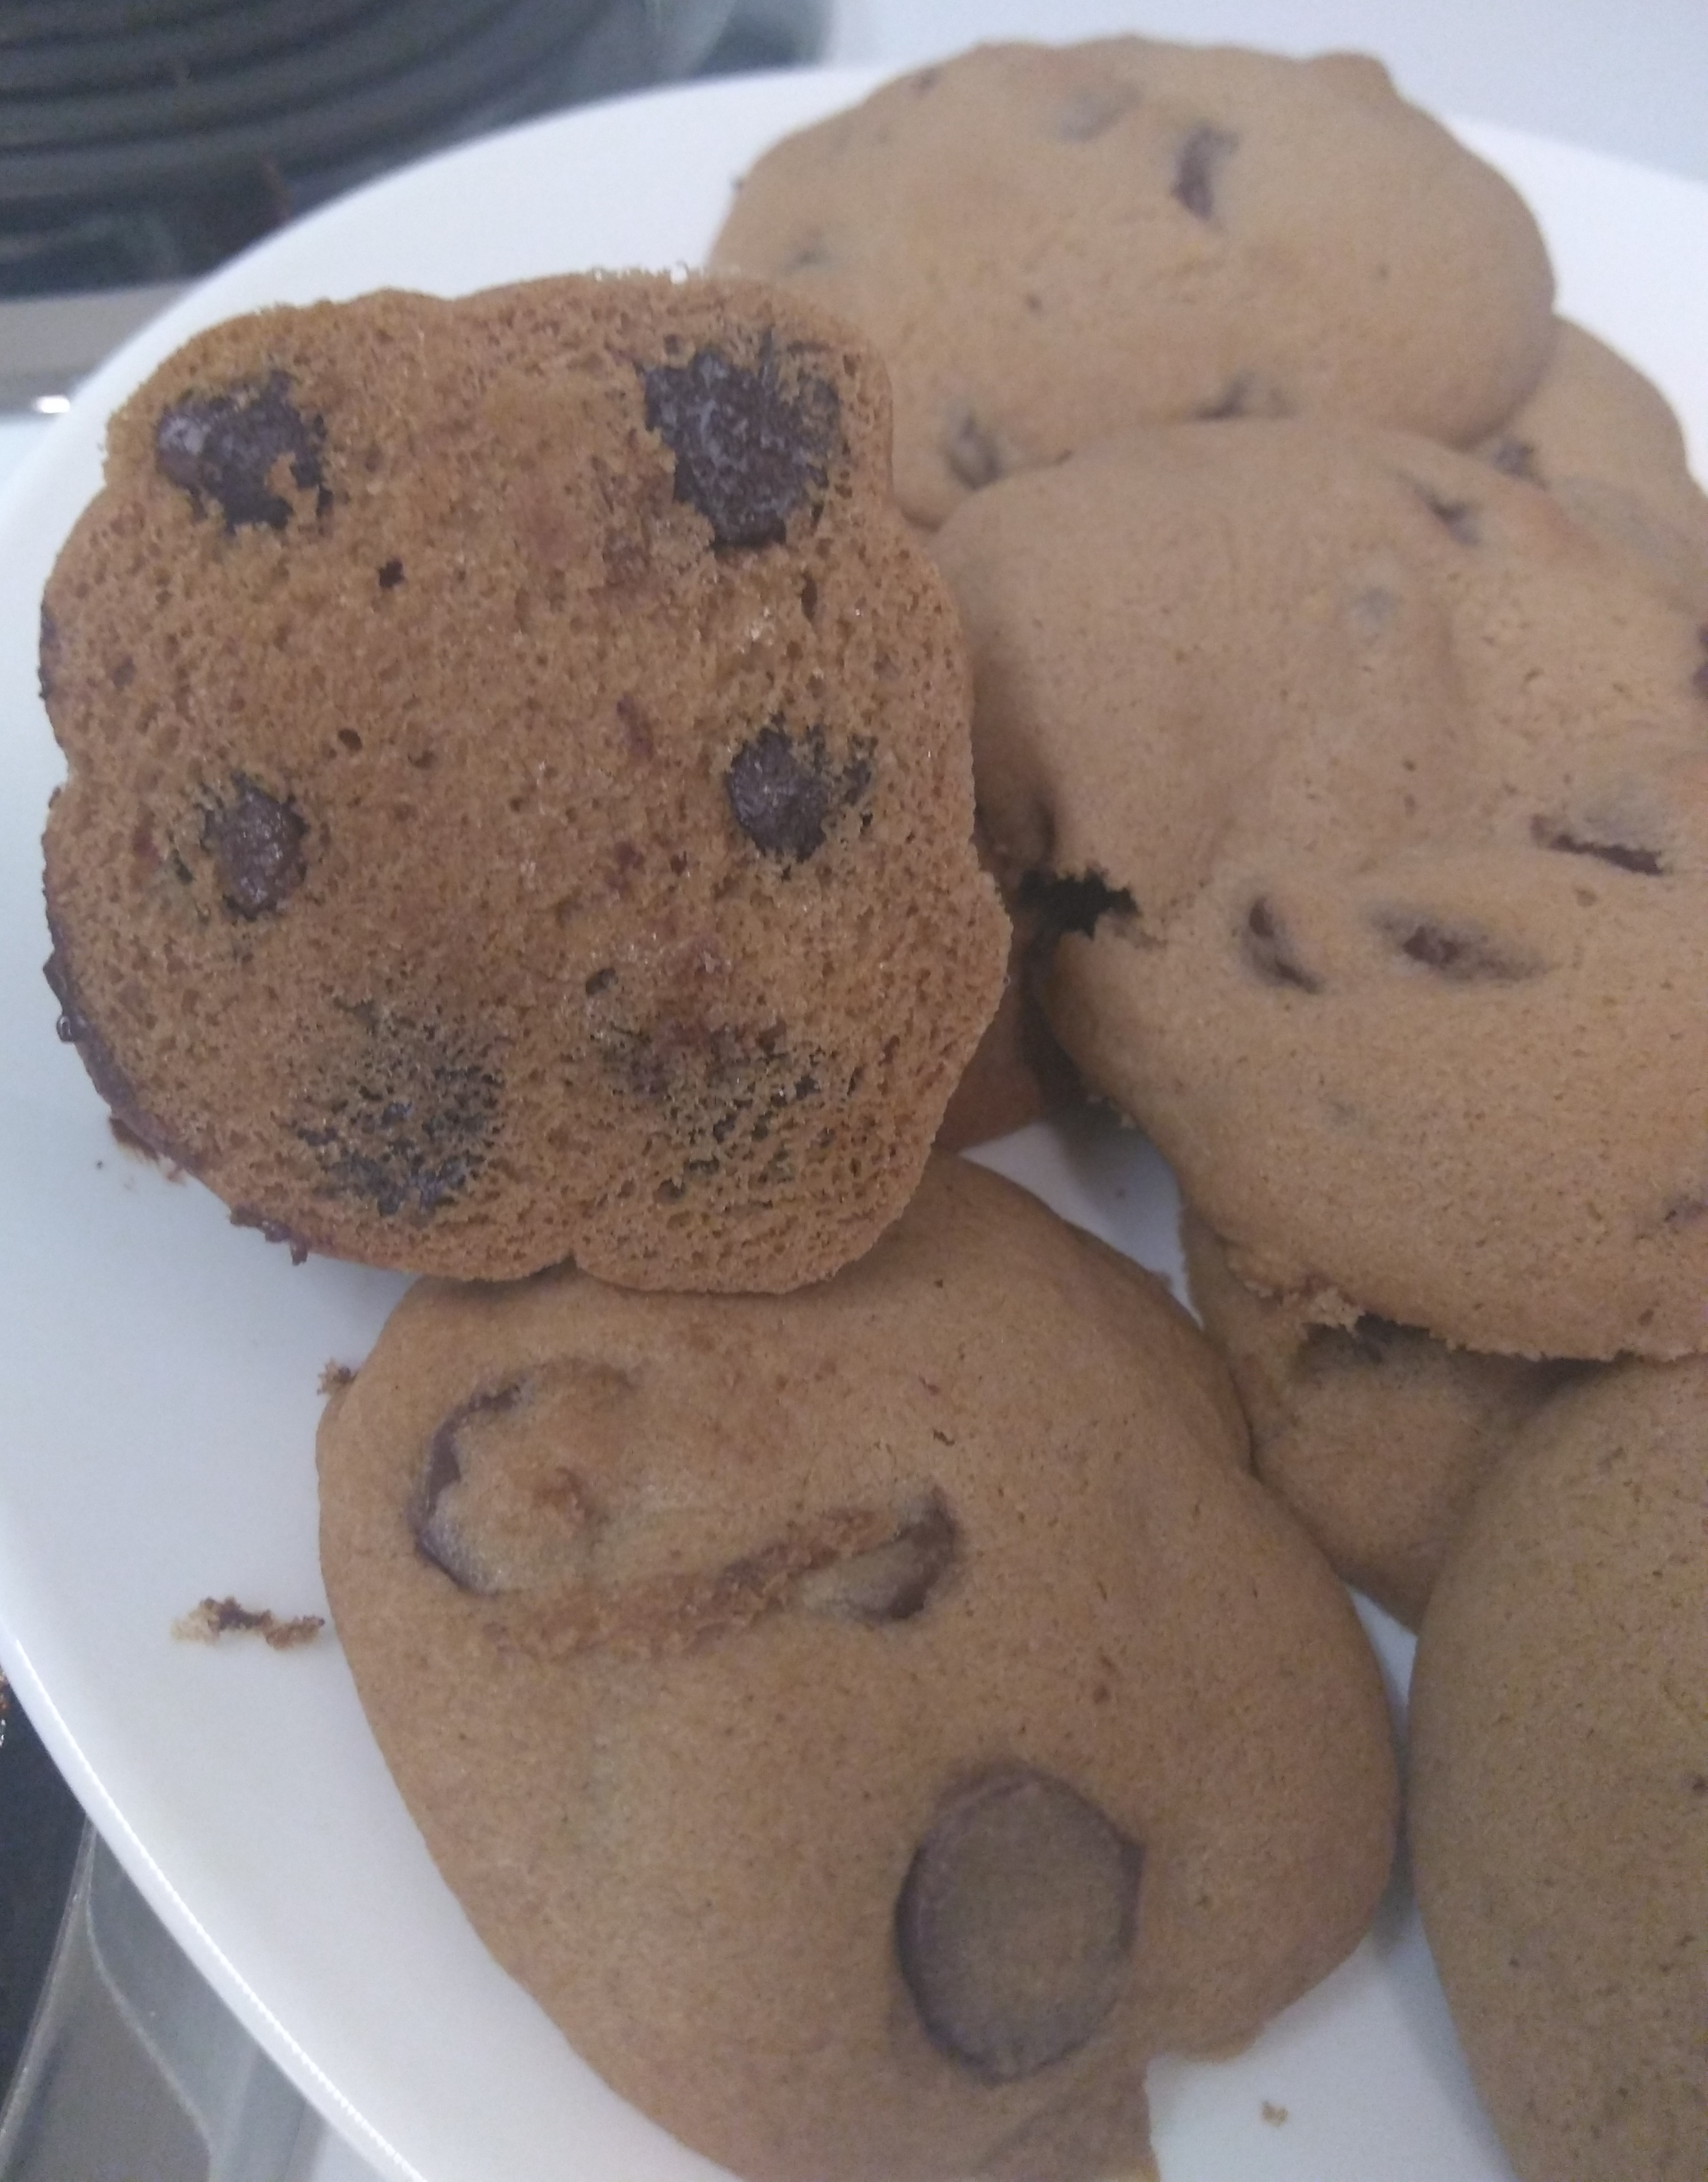
\includegraphics[width=0.6\linewidth]{./pics/cookies.jpg}
\caption{This batch was cooked on an "Airbake" brand, hollow, aluminum baking pan on the middle rack.}
\end{center}
\end{figure}


\end{flushleft}
\end{document}
